% JarvisTEC — project report. Compile with pdflatex + bibtex (Overleaf default).
\documentclass[11pt,letterpaper]{article}

\usepackage[utf8]{inputenc}
\usepackage[T1]{fontenc}
\usepackage[english]{babel}
\usepackage[margin=2.5cm]{geometry}
\usepackage{lmodern}
\usepackage{microtype}
\usepackage{graphicx}
\usepackage{booktabs}
\usepackage{tabularx}
\usepackage{array}
\usepackage{longtable}
\usepackage{enumitem}
\usepackage{amsmath}
\usepackage{xcolor}
\usepackage{listings}
\usepackage{tikz}
\usetikzlibrary{arrows.meta,positioning,shapes.geometric,fit,calc}
\usepackage[hidelinks]{hyperref}

\lstset{
  basicstyle=\ttfamily\small,
  breaklines=true,
  frame=single,
  columns=fullflexible,
  keepspaces=true,
  showstringspaces=false,
  backgroundcolor=\color{gray!8},
}

\newcolumntype{L}{>{\raggedright\arraybackslash}X}
\newcommand{\code}[1]{\texttt{#1}}
\newcommand{\jarvis}{JarvisTEC}

\title{\jarvis{}: a voice and vision assistant over ten machine learning models}

\begin{document}

% Cover page in the TEC format: logo, institution, course, professor, title, members.
% Everything centered, 12 pt, no bold, triple spacing.
\begin{titlepage}
  \centering
  \setlength{\baselineskip}{3\baselineskip}
  
\includegraphics[width=3.7in,height=0.7in]{figures/tec-logo.jpeg}\par
  Instituto Tecnol\'ogico de Costa Rica\par
  Campus Tecnol\'ogico Local San Carlos\par
  Curso:\par
  Inteligencia Artificial\par
  Profesor:\par
  Efr\'en Jim\'enez Delgado\par
  \jarvis\par
  A voice and vision assistant over ten machine learning models\par
  Integrantes:\par
  Jonathan Sancho Loaiza\par
  Jennifer L\'opez Miranda\par
  Magdaleno G\'omez D\'iaz\par
\end{titlepage}

\tableofcontents
\clearpage

\section{Proposed solution}
\label{sec:solution}

\subsection{Problem statement}

The project asks for a personal assistant that hears the user, reads the
user's face, and answers questions about a set of machine learning problems.
Its scope has four deliverables: an agent that recognises the emotion of the
person from a live camera frame, an agent that turns speech into text and
executes the instruction, at least ten machine learning models chosen from
the list of the course, and a set of spoken commands that run those models.
The models are served by a REST API, and the user talks to them through a
desktop application.

\jarvis{} is the answer to that statement. It is a Spanish-speaking desktop
assistant in which every request follows one path: the microphone records
the user, a speech-to-text model transcribes the audio, an intent parser
decides which of the ten models the sentence refers to and which values it
carries, the REST API runs that model, and the reply is written and spoken
back in a tone that depends on the emotion the webcam read on the user's
face. An animated penguin avatar changes its expression with that emotion.

\subsection{Design decisions}

Three decisions shape the solution and are defended here rather than in the
code.

\paragraph{Everything runs locally.}
The statement allows cloud services from Google or Azure for face and speech
recognition in the first delivery. \jarvis{} does not depend on them: the
emotion classifier is a convolutional network exported to ONNX and run with
\code{onnxruntime} on the CPU, speech-to-text is Whisper
through \code{faster-whisper}, and text-to-speech is Piper with a Mexican
Spanish voice. The only optional cloud call is to Gemini for intent parsing,
and when no key is configured a rule-based parser takes over with the same
contract, so the assistant works offline end to end. This makes the demo
independent of quotas, network and billing, and keeps the user's camera
frames and voice on the machine.

\paragraph{Ten models, one contract.}
Each model is a CRISP-DM notebook that ends by writing a
\code{joblib} bundle with the estimator and everything the API needs to feed
it without retraining: the predictor list, encodings, fill values for
missing inputs, thresholds, class names and training ranges. The API loads
the bundles once at startup and exposes them behind one endpoint shape,
\code{POST /predict/\{model\_name\}}. The application never touches an
estimator; it only speaks JSON. Adding an eleventh model is a notebook, an
adapter and a schema, and the assistant discovers the new schema at startup.

\paragraph{The emotion changes how the answer is said, not what it says.}
The classifier returns one of seven emotions (angry, disgust, fear, happy,
sad, surprise, neutral), the vocabulary of the FER-2013 challenge, which in turn follows Ekman's basic emotions. The prediction of the model is computed first and is
identical whatever the face shows; a tone table then wraps it in a prefix
and a suffix (calm and short for an angry user, cheerful for a happy one).
This keeps the machine learning answer auditable and confines the affective
layer to phrasing.

\subsection{Commands}

The assistant wakes on the word \emph{JarvisTEC} (and the mishearings
Whisper produces for it, such as \emph{Yarvis} or \emph{Yalvis}, all matched on
a word boundary). One sentence per model is enough when it carries every
value the model needs; when a required value is missing the assistant asks
for it and keeps the pending intent across turns. Three example sentences
per model, in Spanish, ship with the application in \code{app/prompts.txt};
Table~\ref{tab:commands} gives one per model.

\begin{table}[htbp]
  \centering
  \small
  \begin{tabularx}{\textwidth}{@{}lL@{}}
    \toprule
    Model & Example command (Spanish, as spoken) \\
    \midrule
    Bitcoin & \emph{JarvisTEC, ¿cuánto va a costar el bitcoin mañana?} \\
    Car price & \emph{JarvisTEC, ¿cuánto vale un carro diesel del 2015 que nuevo costó 10 lakhs, tiene 40 mil kilómetros, un solo dueño, lo vende una agencia y es manual?} \\
    Churn & \emph{JarvisTEC, ¿se va a ir un cliente hombre \ldots contrato mes a mes, factura electrónica, paga con cheque electrónico, lleva 3 meses y paga 95 dólares al mes?} \\
    Wine & \emph{JarvisTEC, ¿qué calidad tiene un vino blanco con 13.5 de alcohol, densidad 0.99, \ldots y 2 de azúcar residual?} \\
    Flight delay & \emph{JarvisTEC, ¿cuánto se va a retrasar el vuelo de American Airlines de Dallas a Chicago el lunes 15 de enero a las 12 del mediodía, con 802 millas?} \\
    Stroke & \emph{JarvisTEC, ¿qué riesgo de derrame tiene un hombre de 68 años, hipertenso, \ldots con glucosa de 140, índice de masa corporal 31 y que dejó de fumar?} \\
    Cirrhosis & \emph{JarvisTEC, ¿tiene cirrosis una mujer de 55 años sin edema, sin ascitis, con hepatomegalia, \ldots plaquetas 200 y protrombina 11?} \\
    Avocado & \emph{JarvisTEC, ¿a cuánto estaría el aguacate orgánico en San Francisco el 10 de septiembre de 2017 con un volumen total de 20 mil \ldots?} \\
    Hepatitis C & \emph{JarvisTEC, ¿qué categoría de hepatitis tiene un hombre de 45 años con albúmina 38, fosfatasa alcalina 60, ALT 30, AST 90, \ldots y proteínas 70?} \\
    Body fat & \emph{JarvisTEC, ¿cuál es mi porcentaje de grasa corporal si mi abdomen mide 90 centímetros, peso 175 libras y mi muñeca mide 18 centímetros?} \\
    \bottomrule
  \end{tabularx}
  \caption{One spoken command per model. The full set, three per model, is in \code{app/prompts.txt}.}
  \label{tab:commands}
\end{table}

\subsection{User interface}

The window (Figure~\ref{fig:ui}) has the avatar and the camera card on the
left and the conversation on the right. The camera card shows the mirrored
webcam feed with the detected face boxed and the emotion and its confidence
written under it. The input row has a single button that is the microphone
while the entry is empty, the send arrow once there is text, and a red
recording indicator while the microphone is open. A status strip at the
bottom reports the microphone, the emotion detector, the API, the
speech-to-text engine and which parser answered (a Gemini model or the
rules). System notices never enter the chat.

\begin{figure}[htbp]
  \centering
  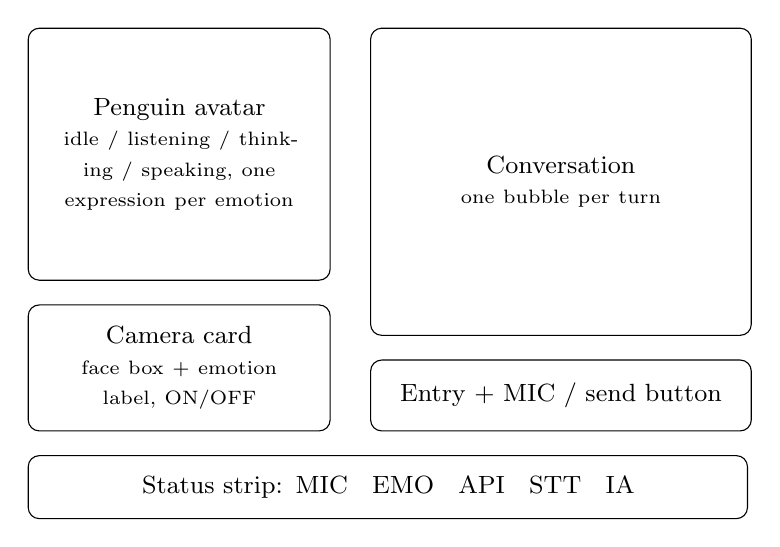
\begin{tikzpicture}[
      every node/.style={font=\small},
      card/.style={draw, rounded corners, text width=3.6cm, align=center},
    ]
    \node[card, minimum height=3.2cm] (avatar) {Penguin avatar\\ \scriptsize idle / listening / thinking / speaking, one expression per emotion};
    \node[card, minimum height=1.6cm, below=0.3cm of avatar] (camera) {Camera card\\ \scriptsize face box + emotion label, ON/OFF};
    \node[card, text width=4.6cm, minimum height=3.9cm, anchor=north west] (chat) at ([xshift=0.5cm]avatar.north east) {Conversation\\ \scriptsize one bubble per turn};
    \node[card, text width=4.6cm, minimum height=0.9cm, below=0.3cm of chat] (input) {Entry + MIC / send button};
    \node[card, text width=8.9cm, minimum height=0.8cm, anchor=north west] (status) at ([yshift=-0.3cm]camera.south west) {Status strip: MIC \; EMO \; API \; STT \; IA};
  \end{tikzpicture}
  \caption{Layout of the \jarvis{} window. \code{Enter} sends typed text, \code{Ctrl+Space} toggles recording, \code{Ctrl+E} toggles the webcam, \code{Esc} quits.}
  \label{fig:ui}
\end{figure}

\section{Machine learning architectures}
\label{sec:architectures}

\subsection{System architecture}

Figure~\ref{fig:pipeline} shows the path of one request. The application is
split into three processes that share only files and HTTP: the notebooks
produce the model bundles, the API serves them, and the desktop application
consumes the API. Inside the application every stage is behind a protocol
(an abstract interface), so the Whisper backend, the Piper backend, the ONNX
emotion detector, the Gemini parser and the HTTP client are each
replaceable without touching the orchestrator.

\begin{figure}[htbp]
  \centering
  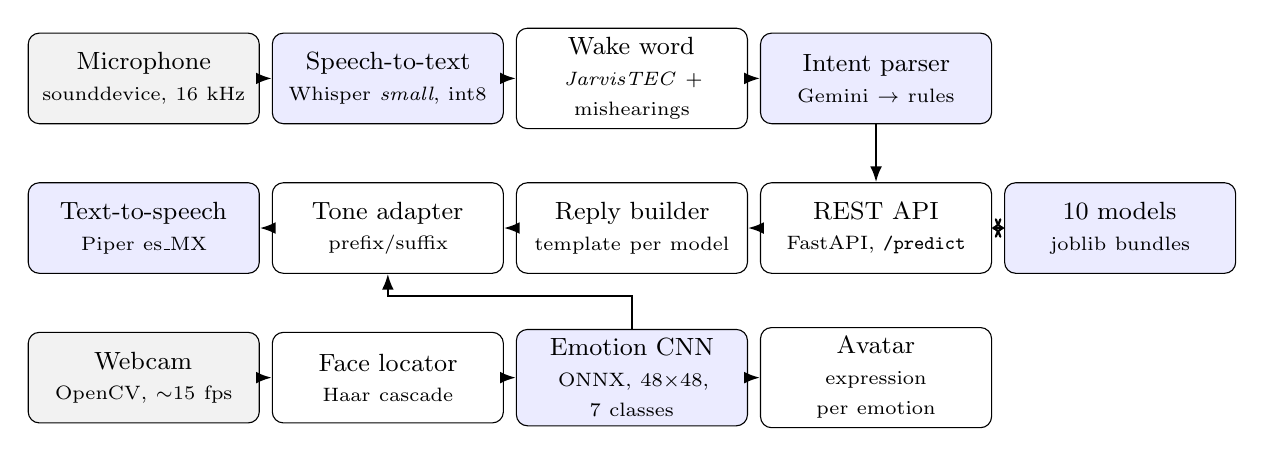
\begin{tikzpicture}[
      x=3.1cm, y=1.9cm,
      every node/.style={font=\small},
      box/.style={draw, rounded corners, align=center, minimum height=1.15cm, text width=2.7cm},
      ml/.style={box, fill=blue!8},
      io/.style={box, fill=gray!10},
      arr/.style={-{Latex[length=2mm]}, thick},
    ]
    \node[io] (mic) at (0,2) {Microphone\\ \scriptsize sounddevice, 16 kHz};
    \node[ml] (stt) at (1,2) {Speech-to-text\\ \scriptsize Whisper \emph{small}, int8};
    \node[box] (wake) at (2,2) {Wake word\\ \scriptsize \emph{JarvisTEC} + mishearings};
    \node[ml] (intent) at (3,2) {Intent parser\\ \scriptsize Gemini $\to$ rules};
    \node[box] (api) at (3,1) {REST API\\ \scriptsize FastAPI, \code{/predict}};
    \node[ml] (models) at (4,1) {10 models\\ \scriptsize joblib bundles};
    \node[box] (reply) at (2,1) {Reply builder\\ \scriptsize template per model};
    \node[box] (tone) at (1,1) {Tone adapter\\ \scriptsize prefix/suffix};
    \node[ml] (tts) at (0,1) {Text-to-speech\\ \scriptsize Piper es\_MX};
    \node[io] (cam) at (0,0) {Webcam\\ \scriptsize OpenCV, $\sim$15 fps};
    \node[box] (face) at (1,0) {Face locator\\ \scriptsize Haar cascade};
    \node[ml] (emo) at (2,0) {Emotion CNN\\ \scriptsize ONNX, 48$\times$48, 7 classes};
    \node[box] (avatar) at (3,0) {Avatar\\ \scriptsize expression per emotion};

    \draw[arr] (mic) -- (stt);
    \draw[arr] (stt) -- (wake);
    \draw[arr] (wake) -- (intent);
    \draw[arr] (intent) -- (api);
    \draw[arr, <->] (api) -- (models);
    \draw[arr] (api) -- (reply);
    \draw[arr] (reply) -- (tone);
    \draw[arr] (tone) -- (tts);
    \draw[arr] (cam) -- (face);
    \draw[arr] (face) -- (emo);
    \draw[arr] (emo) -- (avatar);
    \draw[arr] (emo.north) -- ++(0,0.22) -| (tone.south);
  \end{tikzpicture}
  \caption{One request through \jarvis{}. Shaded boxes are learned models. Typed text enters at the wake-word stage and follows the same path.}
  \label{fig:pipeline}
\end{figure}

\subsection{Perception agents}

\paragraph{Facial emotion agent.}
Every 2 seconds the camera worker takes the current frame, converts it to
grayscale and runs the Viola--Jones Haar cascade
(\code{haarcascade\_frontalface\_alt}) to locate the largest frontal face,
rejecting boxes under $60\times60$ pixels to avoid glare and texture
patches. The crop is resized to $48\times48$, scaled to $[0,1]$ and fed to a
VGG-style convolutional network: five blocks of
$3\times3$ convolutions with ReLU (64, 128, 256, 512 and 512 filters, two or
three convolutions per block), each block closed by batch normalisation and
$2\times2$ max pooling, then a dense layer of 128 units with dropout 0.2 and
a softmax over the seven classes. The network was trained on FER-2013 and reused from an earlier course project; for this
project the Keras weights were exported once to ONNX so that inference runs
with \code{onnxruntime} on the CPU with two threads and does not starve the
interface. The winning class always drives the avatar and the tone; with
seven classes a webcam reading rarely exceeds 50\,\% probability, so the
confidence is shown for information only. The reading is repeated every two
seconds and the face box is redrawn on every frame in between.

\paragraph{Speech agent.}
\code{Ctrl+Space} or the microphone button opens a 16\,kHz mono recording;
pressing again closes it. The audio goes to Whisper \emph{small} through \code{faster-whisper} (CTranslate2), loaded
in int8 on the CPU with Spanish fixed as the language. The transcript then
follows exactly the same path as typed text: wake-word check, intent
parsing, prediction, reply. Whisper's typical mishearings of the wake word
are part of the wake-word table, and the Gemini prompt is told the text may
come from speech so it can recover \emph{días} from \emph{dientes}.

\paragraph{Intent parser.}
The parser turns a Spanish sentence into
\code{(model\_name, fields, missing)}. With a key configured, Gemini is asked
for a JSON object under a system instruction that carries the catalogue of
the ten models (a one-line description, Spanish synonyms and per-model
inference rules) and the JSON schema of every request body, which the
application reads from the API's OpenAPI document at startup. Models are
tried in a chain and a model whose quota is exhausted (429) or that was
retired (404) is skipped for the rest of the session. Without a key, or on
any Gemini failure, a rule-based parser with one field extractor per model
(keyword lookup tables, Spanish number words, dates, airline and city codes)
produces the same structure. Whichever parser answered is shown in the
status strip.

\paragraph{Dialogue.}
The orchestrator records the turn, resolves the intent against the pending
one (so an answer to ``which airline?'' completes the flight request from
the previous turn), asks for the next missing required field if any, or
posts the request body to the API and renders the answer through a per-model
reply template. The tone adapter wraps the text according to the last
emotion, and the speaking worker synthesises it with Piper
(\code{es\_MX-claude-high}, 22\,kHz). Starting a new recording interrupts the
voice.

\subsection{The ten models}

Table~\ref{tab:models} lists the ten problems, their datasets, the technique
required by the course for each and the target. Each one is developed in
its own notebook with the six CRISP-DM phases: problem
analysis, data understanding, exploration and preparation, modelling,
evaluation and deployment (the saved bundle plus a reload test). Every
notebook builds the literal model the task asks for first, and when the data
call for a deviation (a logarithm, a regrouped target, a balanced class
weight) that second model is built next to it and the choice is defended
with the metrics of both.

\begin{table}[htbp]
  \centering
  \small
  \begin{tabularx}{\textwidth}{@{}c>{\ttfamily}lLLL@{}}
    \toprule
    \# & Notebook & Dataset (source) & Technique & Target \\
    \midrule
    1 & bitcoin\_price\_regression & Bitcoin daily prices 2013--2017 (Kaggle, team-ai) & ARIMA & closing price, next days \\
    2 & car\_price\_regression & 301 used cars, India (Kharwal) & multiple linear regression & selling price (lakhs) \\
    3 & telecom\_churn\_classification & IBM Telco churn, 7\,043 customers & neural network (MLP) & churn yes/no \\
    4 & wine\_quality\_classification & Vinho verde, 6\,497 wines & $k$ nearest neighbours & quality band \\
    5 & flight\_delay\_regression & BTS airline delays 2008, 1.9\,M flights & decision tree & arrival delay (min) \\
    6 & stroke\_classification & Stroke prediction, 5\,110 people (fedesoriano) & logistic regression & stroke yes/no \\
    7 & cirrhosis\_type\_classification & Mayo PBC trial, 418 patients & support vector machine & cirrhosis stage \\
    8 & avocado\_price\_regression & Hass Avocado Board retail scans 2015--2018 & random forest & average price (USD) \\
    9 & hepatitis\_type\_classification & HCV blood panels, 615 people & Gaussian naive Bayes & donor / hepatitis / fibrosis / cirrhosis \\
    10 & body\_fat\_regression & 252 men & multiple linear regression & body fat (\%) \\
    \bottomrule
  \end{tabularx}
  \caption{The ten models, in the order of the repository. All datasets are downloaded by the notebooks through \code{kagglehub} or a public URL.}
  \label{tab:models}
\end{table}

\subsection{Serving architecture}

The API is a FastAPI service with one adapter per model. Each adapter knows
how to turn a validated request body into the row the estimator expects
(filling optional fields with the notebook's fill value, applying the
notebook's encodings and transformations) and how to turn the estimator's
output into the response (label, probability and threshold for classifiers;
value and units for regressions; a list of \code{\{date, price, lower,
upper\}} for the forecast). Requests are validated by Pydantic schemas that
mirror the notebook's predictor list, and regressions attach a warning when
an input falls outside the training range, since a fitted line has no
information beyond it. Endpoints, request bodies and example calls are listed
in Appendix~\ref{app:api}.

\section{Justification and explanation of the models}
\label{sec:justification}

Each subsection says what the model is asked, why the technique fits, what
had to be done to the data, and which of the models built in the notebook
was kept and why. The numbers are the ones printed by the executed
notebooks in the repository.

\subsection{Bitcoin price: ARIMA}

\paragraph{The question.} What will bitcoin cost in the next few days?

\paragraph{Why ARIMA.} There are no predictors here, only the history of
the price, and ARIMA is the technique of the course for forecasting a
series from its own past.

\paragraph{What the data needed.} The price grew twenty-fold over the four
years, and its daily jumps grew with it: a 10\,\% move was 20 dollars in 2015
and 250 in 2017. ARIMA needs a series with a stable mean and a stable
spread, so two steps were taken. Taking the logarithm makes the spread
stable, because it turns dollar changes into percentage changes. Taking
the difference between one day and the next removes the trend. After those
two steps the statistical test for stationarity passes.

\paragraph{What the model found.} The daily percentage change of bitcoin
has almost no memory: knowing today's change says almost nothing about
tomorrow's. That is what economists call a random walk, and it means the
best guess for tomorrow is roughly today's price. The notebook tried
sixteen ARIMA orders and kept the one with the best AIC score,
ARIMA(3,1,3), but none of its coefficients is statistically different from
zero, so it is really a random walk with a few small extra terms.

\paragraph{What is kept.} The ARIMA is kept because, unlike a plain
``same as today'' answer, it gives a range around the forecast that widens
with the horizon. The assistant reads out the number and the range, and
Section~\ref{sec:results} shows honestly that the number itself is no
better than repeating the last price.

\subsection{Used car price: multiple linear regression}

\paragraph{The question.} How much does a used car sell for, given its
showroom price, year, mileage, fuel, seller and transmission?

\paragraph{Why linear regression.} A dealer wants to know how much each
fact is worth, for example how much a year of age costs. A linear
regression gives exactly that: one coefficient per fact, in units of
price.

\paragraph{What the data needed.} Most cars are cheap and a few are very
expensive, so prices are lopsided. Fitting the price directly, the model
gets the expensive cars badly wrong and its errors grow with the price.
Fitting the logarithm of the price instead, with the logarithm of the
showroom price and of the mileage, fixes that; the coefficients then read
as percentages, which is the natural way to talk about depreciation.

\paragraph{What is kept.} The logarithmic model, with an $R^2$ of 0.954
against 0.807 for the direct model and half the error. Cars outside the
range seen in training (a much more expensive or much older car) are not
predicted, because a straight line knows nothing beyond its data. The
coefficient for CNG rests on two cars and is reported as unknown.

\subsection{Telecom churn: neural network}

\paragraph{The question.} Will this customer cancel the service?

\paragraph{Why a neural network.} A multilayer perceptron can combine the
30 facts about a customer (contract, services, bill, tenure) in ways a
straight line cannot. The network has two hidden layers of 32 and 16
neurons and one output neuron that gives a probability.

\paragraph{Why ReLU.} The activation of the hidden neurons is set
explicitly. The notebook tries the four that scikit-learn offers
(identity, logistic, tanh and ReLU) with the same architecture, on the
training data alone, and they land within one standard deviation of each
other: a cross-validated AUC between 0.830 and 0.839 with a fold moving it
by about 0.014. The identity row matches the rest, which says the churn
signal is largely linear, but a network with no non-linearity is a logistic
regression and is not kept. Among the non-linear three ReLU is kept because
its gradient does not fade on the positive side, and the other two buy
nothing measurable here in exchange for their saturating sums.

\paragraph{What the data needed.} Only about one customer in four leaves,
so the network learns to say ``stays'' most of the time: at the usual cut
of 0.5 it reaches 79\,\% accuracy but catches only half of the customers
who leave. The notebook sweeps the threshold and shows that the ranking
behind the probabilities is good (AUC 0.84): lowering the cut to 0.3 finds
three leavers out of four at the price of twice the false alarms.

\paragraph{What is kept.} The network at the 0.5 threshold, which is the
most accurate cut, with the probability stored so the company can lower the
threshold when a retention call is cheap next to a lost customer. The
weak number is stated plainly: about four customers in ten on the list
would not have left, so the list is a set of customers worth a call, not a
verdict.

\subsection{Wine quality: $k$ nearest neighbours}

\paragraph{The question.} How good is a wine, from its laboratory sheet?

\paragraph{Why $k$-NN.} It needs no equation: to score a new wine it looks
up the $k$ most similar wines in the training set and takes the most common
score among them.

\paragraph{What the data needed.} ``Similar'' means close in every
measurement, but the measurements use very different scales (sulphur
dioxide in the hundreds, density around 1). Without putting them on the
same scale the distance is decided by sulphur dioxide alone, so every
measurement was standardised. The second problem is the target: scores go
from 3 to 9 but almost every wine is a 5, 6 or 7, and a vote among
neighbours never picks the rare scores. Grouping the scores into low,
medium and high gives every class enough wines to win a vote.

\paragraph{What is kept.} The three-band model with $k = 39$. It gets the
band right 59\,\% of the time, against 44\,\% for always answering
``medium'', and its mistakes are between neighbouring bands. The honest
reading is that the laboratory sheet explains only part of what tasters
score, so the assistant gives a band, not a number.

\subsection{Flight delay: decision tree}

\paragraph{The question.} How late will this flight arrive?

\paragraph{Why a decision tree.} A tree asks a chain of yes/no questions
(``does it depart after 5 pm?'', ``is it this airline?'') and predicts the
average delay of the flights that answered the same way. Its rules can be
read, so the assistant could explain why it expects a delay.

\paragraph{What the data needed.} The file contains the departure delay
of every flight. A tree that reads it predicts the arrival delay almost
perfectly ($R^2$ of 0.95), but that is cheating: if you already know the
plane left forty minutes late you do not need a model. The honest tree only
reads what is known before leaving home: airline, route, month, weekday,
scheduled hour and distance.

\paragraph{What is kept.} The honest tree, with an $R^2$ of 0.05 and an
average error of 36 minutes. The notebook says plainly that this is a weak
model, and explains why: delays come from weather, breakdowns, late
inbound aircraft and airport congestion, none of which is in the schedule.
The assistant gives the expected delay together with that error.

\subsection{Stroke risk: logistic regression}

\paragraph{The question.} Is this person at risk of a stroke?

\paragraph{Why logistic regression.} It turns a set of facts (age, blood
pressure, heart disease, glucose, body mass, smoking) into a probability
between 0 and 1, and a threshold on that probability gives a yes or no.

\paragraph{What the data needed.} Only 1 person in 20 in the file had a
stroke. Trained as is, the model says ``no'' to almost everyone: 95\,\%
accuracy, but it finds 2 strokes out of 62. For a screening tool that is
useless. Telling the model that a missed stroke weighs as much as the
nineteen healthy people it is outnumbered by (balanced class weights)
fixes it.

\paragraph{What is kept.} The balanced model. It finds 50 of the 62
strokes, at the cost of sending about 300 healthy people out of 1\,216 to a
check-up. Age matters five times more than any other fact. Because only
about one positive in seven is a real stroke, the assistant presents a
positive answer as a reason to see a doctor, never as a diagnosis.

\subsection{Cirrhosis stage: support vector machine}

\paragraph{The question.} How advanced is this patient's liver disease,
from blood tests and physical signs, without a biopsy?

\paragraph{Why an SVM.} It draws the boundary between classes that leaves
the widest gap on each side, and with the radial kernel that boundary can
curve. Because it measures distances between patients, all the tests had to
be put on the same scale first, and its two settings ($C$ and $\gamma$)
were chosen by cross-validation.

\paragraph{What the model found.} Telling apart the four stages is not
possible from these data: stages 2 and 3 have the same typical values on
almost every test, and no setting of the model got above 45\,\% balanced
accuracy. What the tests do show is whether the patient has reached
cirrhosis (stage 4) or not.

\paragraph{What is kept.} The two-class model, cirrhosis or earlier, right
about three times in four. The four-stage model is saved next to it so the
API can still answer with a stage, with its limitation attached. The data
come from a clinical trial of the 1970s and 1980s, mostly women, so the
model is a screen, not a diagnosis.

\subsection{Avocado price: random forest}

\paragraph{The question.} What will an avocado cost in a given city, for
a given type (organic or conventional) and week?

\paragraph{Why a random forest.} A single decision tree memorises its
training data: grown without limits it is perfect on the rows it saw and
much worse on new ones. A forest grows hundreds of trees on random
samples and averages them, which keeps what the trees learn and cancels
what they memorise.

\paragraph{What the model found.} The forest of 200 trees explains 90\,\%
of the price with an average error of nine cents, and its out-of-bag
score agrees. The type of avocado is by far the most important fact
(organic costs about half a dollar more), followed by the quantities sold
and the season.

\paragraph{What is kept.} The forest, with one warning. Trained on
2015--2017 and asked about 2018, it explains only 41\,\% of the price,
because a forest cannot guess a year it has never seen. So it is used to
look up the expected price for a region, type and season, not to forecast
next year.

\subsection{Hepatitis C category: naive Bayes}

\paragraph{The question.} Does this blood panel look like a healthy
donor, hepatitis, fibrosis or cirrhosis?

\paragraph{Why naive Bayes.} It computes, for each category, how likely
the observed lab values are, and picks the most likely category. It works
well with few examples, which matters here: the file has 533 donors but
only 24, 21 and 30 sick patients.

\paragraph{What the data needed.} The Gaussian version assumes each lab
value follows a bell curve within each category. Liver enzymes do not:
most values are small and a few are huge. Taking the logarithm of every
lab value makes them bell-shaped and raises the balanced accuracy from
0.65 to 0.71.

\paragraph{What is kept.} The logarithmic model. It separates donors from
patients almost perfectly and recognises cirrhosis four times out of five,
but it confuses hepatitis and fibrosis with each other about half the
time, so the assistant reads either of those as ``early liver disease''.
Because the sick groups are so small, the numbers come from five-fold
cross-validation rather than a single test set.

\subsection{Body fat: multiple linear regression}

\paragraph{The question.} What is a person's body fat percentage, from
measurements taken with a tape and a scale?

\paragraph{Why linear regression.} The reference method (underwater
weighing) is expensive; a formula with a few readable coefficients is what
a trainer can actually use.

\paragraph{What the data needed.} The file has thirteen measurements, but
they mostly say the same thing: a bigger man has a bigger chest, waist,
hip and thigh, all at once. When predictors repeat each other, a
regression cannot decide how to share the effect between them and its
coefficients become meaningless, some even with the wrong sign. The
\code{Density} column was dropped because the target is computed from it.
Two impossible rows (a man 75 centimetres tall, a body fat of exactly 0)
were removed.

\paragraph{What is kept.} A model with three measurements: abdomen,
weight and wrist. It is as accurate as the model with all thirteen
(average error of 3.9 points of fat against 3.8, on a test set too small to
tell the difference) and its three coefficients can be read and trusted.
The limitation is the error itself: a man predicted at 20\,\% may be at 16
or 24, enough to place him in a broad category but not to follow a diet
week by week.

\section{Analysis of results}
\label{sec:results}

\subsection{Model metrics}

Tables~\ref{tab:forecast} to \ref{tab:recall} gather the metrics of the
model kept in each notebook, next to the literal model built first when the
two differ. Every figure is computed on rows the model never saw: a 25\,\%
random test split for most notebooks, a chronological hold-out for the two
series, and five-fold cross-validation for hepatitis, whose sick classes are
too small for a single split.

\begin{table}[htbp]
  \centering
  \small
  \begin{tabular}{@{}llrrr@{}}
    \toprule
    Forecast & Window & MAE (USD) & RMSE (USD) & MAPE (\%) \\
    \midrule
    ARIMA(3,1,3) & 30 validation days & 210.7 & 246.6 & 8.4 \\
    Naive (last price) & 30 validation days & 214.1 & 249.7 & 8.6 \\
    ARIMA(3,1,3) & 7 unseen days, August 2017 & 236.1 & 282.1 & 7.6 \\
    Naive (last price) & 7 unseen days, August 2017 & 233.2 & 284.9 & 7.5 \\
    \bottomrule
  \end{tabular}
  \caption{Bitcoin forecast against the naive forecast on the two hold-outs.}
  \label{tab:forecast}
\end{table}

\begin{table}[htbp]
  \centering
  \small
  \begin{tabularx}{\textwidth}{@{}lLrrrl@{}}
    \toprule
    Model & Test rows & $R^2$ & MAE & RMSE & Units \\
    \midrule
    Car price, log model (kept) & 72 cars in range & 0.954 & 0.65 & 1.03 & lakhs \\
    Car price, raw price & 72 cars in range & 0.807 & 1.23 & 2.11 & lakhs \\
    Flight delay, schedule only (kept) & 50\,000 flights & 0.050 & 36.0 & 56.6 & minutes \\
    Flight delay, with departure delay & 50\,000 flights & 0.952 & 8.9 & 12.7 & minutes \\
    Avocado, random forest (kept) & 4\,563 random weeks & 0.898 & 0.091 & 0.128 & USD \\
    Avocado, single tree, depth 10 & 4\,563 random weeks & 0.749 & 0.146 & 0.201 & USD \\
    Avocado, random forest & 1\,296 weeks of 2018 & 0.410 & 0.188 & 0.235 & USD \\
    Body fat, 3 predictors (kept) & 59 men & 0.583 & 3.87 & 4.64 & \% fat \\
    Body fat, all 13 predictors & 59 men & 0.602 & 3.83 & 4.53 & \% fat \\
    \bottomrule
  \end{tabularx}
  \caption{Regression results. The avocado forest's out-of-bag $R^2$ is 0.893; the adjusted $R^2$ of the two body fat models is 0.561 and 0.487.}
  \label{tab:regressions}
\end{table}

\begin{table}[htbp]
  \centering
  \small
  \begin{tabular}{@{}llrrrrr@{}}
    \toprule
    Model & Test rows & Acc. & Sens. & Spec. & Prec. & AUC \\
    \midrule
    Churn, MLP oversampled (kept) & 1\,761 customers & 0.755 & 0.745 & 0.759 & 0.527 & 0.831 \\
    Churn, MLP as is & 1\,761 customers & 0.790 & 0.529 & 0.885 & 0.624 & 0.840 \\
    Stroke, balanced logistic (kept) & 1\,278 people & 0.751 & 0.806 & 0.748 & 0.140 & 0.843 \\
    Stroke, plain logistic & 1\,278 people & 0.952 & 0.032 & 0.999 & 0.667 & 0.845 \\
    \bottomrule
  \end{tabular}
  \caption{Binary classifiers at the 0.5 threshold.}
  \label{tab:binary}
\end{table}

\begin{table}[htbp]
  \centering
  \small
  \begin{tabularx}{\textwidth}{@{}lLlrr@{}}
    \toprule
    Model & Question & Evaluated on & Acc. & Bal.\ acc. \\
    \midrule
    Wine, $k$-NN, $k=39$ (kept) & 3 bands & 1\,333 test wines & 0.589 & 0.547 \\
    Wine, $k$-NN, $k=5$ & 7 scores & 1\,333 test wines & 0.513 & 0.230 \\
    Cirrhosis, SVM (kept) & stage 4 or earlier & 103 test patients & 0.777 & 0.758 \\
    Cirrhosis, SVM tuned & stages 1 to 4 & 103 test patients & 0.447 & 0.424 \\
    Hepatitis, Gaussian NB, log labs (kept) & 4 categories & 608 people, 5-fold CV & 0.934 & 0.709 \\
    Hepatitis, Gaussian NB, raw labs & 4 categories & 608 people, 5-fold CV & 0.914 & 0.653 \\
    \bottomrule
  \end{tabularx}
  \caption{Multi-class classifiers.}
  \label{tab:multiclass}
\end{table}

\begin{table}[htbp]
  \centering
  \small
  \begin{tabularx}{\textwidth}{@{}lL@{}}
    \toprule
    Kept model & Recall by class \\
    \midrule
    Wine, 3 bands & low 0.66, medium 0.63, high 0.35 \\
    Cirrhosis, stage 4 or earlier & earlier stages 0.82, cirrhosis 0.69 \\
    Hepatitis, 4 categories & donor 0.98, hepatitis 0.58, fibrosis 0.48, cirrhosis 0.80 \\
    \bottomrule
  \end{tabularx}
  \caption{Per-class recall of the kept multi-class models.}
  \label{tab:recall}
\end{table}

\subsection{Reading the numbers}

\paragraph{Three models are strong.}
The car price model explains 95\,\% of the variance of the log price with
an error of 0.65 lakhs, the avocado forest explains 90\,\% with an error of
nine cents on a random split, and the hepatitis classifier tells a donor
from a patient with a recall of 0.98. All three are recommended to the
assistant without reservation inside the range of their training data.

\paragraph{Four models are useful screens.}
Churn (AUC 0.83), stroke (AUC 0.84), cirrhosis-or-not (balanced accuracy
0.76) and body fat (error of 3.9 points) separate their classes or place a
person in a broad band, and each notebook states the precision or the error
that makes its answer a reason to look closer rather than a verdict. In
every one of them the decision that mattered was not the estimator but the
treatment of the imbalance or of the multicollinearity: balanced weights
turned a stroke model that found 2 of 62 strokes into one that finds 50,
oversampling did the same for churn, and dropping ten collinear
circumferences made the body fat slopes readable at no measurable cost.

\paragraph{Three models are honest negatives.}
The ARIMA does not beat the naive forecast on either hold-out; the
difference is three dollars on a price of 2\,500 and changes sign between
the two windows, which is the result the flat autocorrelation announced:
the daily return of bitcoin has no usable memory. The wine model misplaces
four wines in ten because the laboratory sheet explains only part of a
tasting score. The flight tree reaches an $R^2$ of 0.05 because the causes
of delay are absent from the schedule. In all three the literal, accurate
looking alternative (an ARIMA judged by its in-sample AIC, a tree that
reads the departure delay) was built, shown, and rejected with the reason.
The project treats reporting these outcomes as part of the scientific
method rather than as failures to hide: the assistant tells the user the
band around the bitcoin forecast, the band rather than the score for wine,
and the 36-minute average error next to any delay.

\paragraph{Evaluation design matters as much as the model.}
The avocado forest drops from $R^2 = 0.90$ on a random split to $0.41$ on
the weeks of 2018, because a random split of a set of time series lets the
model interpolate between neighbouring weeks. The hepatitis model is scored
by cross-validation because its sick classes have 21 to 30 people. The car
and body fat models exclude test rows outside the training range, and the
API carries that rule into production as a warning on every out-of-range
request.

\subsection{Application and API}

All ten models are served by the API and reachable from the assistant by
voice and by text; the repository ships three spoken sentences per model
that resolve in a single turn with Gemini and also with the local rules.
The rule-based parser is covered by 82 unit tests
(\code{app/intents/rules/tests}) that pass on the current revision; they
check that every shipped prompt resolves locally without Gemini and that the
extractors of the car price and stroke models read numbers, dates, Spanish
number words and synonyms correctly.

The perception agents were validated by use rather than by a held-out set,
since no labelled corpus of the team's faces or voices exists. Three
observations from that use shaped the code. First, a USB webcam's first
frames are nearly black while its exposure settles, so ten frames are
discarded on open to avoid reporting ``no face''. Second, Whisper
\emph{small} in int8 runs at usable latency on a laptop CPU, and it
mishears the wake word in a handful of stable ways, which are now in the
wake-word table. Third, with
seven emotion classes the winning probability of a webcam frame is often
below 0.5 and flips between neutral and a neighbour, so the emotion is
sampled every two seconds rather than every frame, and only the winner
drives the tone and the avatar.

\subsection{Limitations and future work}

The emotion classifier was reused from a previous course project and not
retrained; its accuracy on FER-2013 was not re-measured here and its
behaviour on the team's faces was only observed. A retraining on FER-2013
with a held-out evaluation, or a lighter architecture, would let the
notebook of that model join the other ten. The flight and wine models
would need data that is not in their files (weather, tasters). The bitcoin
model would need exogenous predictors to beat a random walk, and the
literature suggests those gains are small. Whisper \emph{small} is a
compromise between latency and accuracy on CPU; a GPU or the \emph{medium}
model would cut mishearings. Finally, the Gemini parser depends on a
free-tier quota, which is why the local rules exist and why the model chain
skips exhausted models for the rest of the session.


\clearpage
\appendix
\section{Repository and reproduction}
\label{app:repo}

The repository is at \url{https://github.com/Jonathansl17/jarvis}. Its
layout:

\begin{lstlisting}
notebooks/   one folder per model, each with its executed CRISP-DM notebook
models/      one .joblib bundle per model, written by the notebooks, read by the API
             plus facial_emotion_cnn.onnx and haarcascade_frontalface_alt.xml
api/         FastAPI service, one adapter and one schema per model
app/         JarvisTEC desktop assistant (CustomTkinter, whisper, Piper, OpenCV)
docs/        this document (LaTeX)
\end{lstlisting}

\paragraph{Notebooks.}
Every notebook downloads its dataset with \code{kagglehub} or from a public
URL, so it runs unchanged in Google Colab and locally, and its last cells
write \code{models/<name>.joblib} and reload it for a sanity prediction.

\begin{lstlisting}[language=bash]
python3 -m venv env && source env/bin/activate
pip install -r notebooks/requirements.txt
jupyter notebook notebooks/
\end{lstlisting}

\paragraph{API.}
\begin{lstlisting}[language=bash]
pip install -r api/requirements.txt
cd api && uvicorn app.main:app --host 0.0.0.0 --port 8000
\end{lstlisting}
Interactive documentation at \url{http://localhost:8000/docs}. Configuration
through the environment variables \code{MODELS\_DIR}, \code{HOST} and
\code{PORT}.

\paragraph{Application.}
\begin{lstlisting}[language=bash]
pip install -r app/requirements.txt
cp app/.env.example app/.env     # optional GEMINI_API_KEY, API_BASE_URL
python -m app                    # with the API running
\end{lstlisting}
The first run downloads Whisper \emph{small} (about 500\,MB) and the Spanish
Piper voice (about 60\,MB). Other variables: \code{GEMINI\_MODELS},
\code{MODELS\_DIR}, \code{PIPER\_CACHE\_DIR}, \code{CAMERA\_ENABLED},
\code{TTS\_ENABLED}. The same steps work on Windows with \code{py -m venv env}
and \code{env\textbackslash Scripts\textbackslash activate}.

\paragraph{Tests.}
\begin{lstlisting}[language=bash]
python -m unittest discover -s app -p "test_*.py" -t .
\end{lstlisting}

\section{REST API}
\label{app:api}

\begin{table}[htbp]
  \centering
  \small
  \begin{tabularx}{\textwidth}{@{}llL@{}}
    \toprule
    Method & Path & Purpose \\
    \midrule
    GET & \code{/health} & liveness, no model lookup \\
    GET & \code{/models} & names of the loaded models \\
    GET & \code{/models/\{model\_name\}/schema} & JSON schema of that model's request body \\
    POST & \code{/predict/\{model\_name\}} & runs one model on a JSON body \\
    \bottomrule
  \end{tabularx}
  \caption{Endpoints of the API.}
\end{table}

Optional fields (\code{null} or omitted) are filled with the value the
notebook used for missing data. Classifiers answer with \code{label},
\code{probability} and the \code{threshold} applied; regressions answer with
the predicted value in the units of the notebook and \code{meta.warnings}
when an input falls outside the training range; bitcoin answers with a list
of \code{\{date, price, lower, upper\}}. Example calls:

\begin{lstlisting}[language=bash]
curl -X POST localhost:8000/predict/car_price_regression \
  -H 'content-type: application/json' -d '{
  "present_price": 10, "year": 2015, "kms_driven": 40000, "owner": 0,
  "fuel_type": "Diesel", "seller_type": "Dealer", "transmission": "Manual"}'

curl -X POST localhost:8000/predict/body_fat_regression \
  -H 'content-type: application/json' -d '{"abdomen": 90, "weight": 175, "wrist": 18}'

curl -X POST localhost:8000/predict/stroke_classification \
  -H 'content-type: application/json' -d '{
  "gender": "Male", "age": 68, "hypertension": true, "heart_disease": false,
  "ever_married": "Yes", "work_type": "Private", "Residence_type": "Urban",
  "avg_glucose_level": 140, "bmi": 31, "smoking_status": "formerly smoked"}'

curl -X POST localhost:8000/predict/hepatitis_type_classification \
  -H 'content-type: application/json' -d '{
  "age": 45, "sex": "m", "ALB": 38, "ALP": 60, "ALT": 30, "AST": 90, "BIL": 30,
  "CHE": 5, "CHOL": 4, "CREA": 80, "GGT": 120, "PROT": 70}'

curl -X POST localhost:8000/predict/wine_quality_classification \
  -H 'content-type: application/json' -d '{
  "type": "white", "alcohol": 13.5, "density": 0.99, "free_sulfur_dioxide": 30,
  "total_sulfur_dioxide": 120, "volatile_acidity": 0.25, "residual_sugar": 2}'

curl -X POST localhost:8000/predict/flight_delay_regression \
  -H 'content-type: application/json' -d '{
  "month": 12, "day_of_month": 19, "day_of_week": 5, "dep_hour": 18,
  "carrier": "AA", "origin": "ORD", "dest": "LAX", "distance": 1745}'

curl -X POST localhost:8000/predict/bitcoin_price_regression \
  -H 'content-type: application/json' -d '{"days": 7}'
\end{lstlisting}

\section{Software stack}
\label{app:stack}

\begin{table}[htbp]
  \centering
  \small
  \begin{tabularx}{\textwidth}{@{}lL@{}}
    \toprule
    Component & Library and version \\
    \midrule
    Notebooks & pandas 3.0.5, scikit-learn 1.9.1, statsmodels 0.15.0, matplotlib 3.11.1, seaborn 0.13.2, kagglehub 1.0.2, joblib 1.6.0 \\
    API & FastAPI 0.141.1, uvicorn 0.52.4, pydantic-settings 2.15.0 \\
    Application & CustomTkinter 6.0.0, faster-whisper 1.2.1, piper-tts 1.8.0, onnxruntime 1.30.0, opencv-python-headless 4.14.0, sounddevice 0.5.6, httpx 0.28.1, google-genai 2.23.0 \\
    Emotion model & VGG-style CNN, Keras weights exported to ONNX; Haar cascade \code{frontalface\_alt} from OpenCV \\
    Speech & Whisper \emph{small}, int8, CTranslate2; Piper voice \code{es\_MX-claude-high} \\
    Intent parsing & Gemini (\code{gemini-3.6-flash}, then \code{gemini-flash-lite-latest}) with a rule-based fallback \\
    \bottomrule
  \end{tabularx}
  \caption{Versions pinned in the three \code{requirements.txt} files.}
\end{table}


\end{document}
